\documentclass[12pt]{report}
\usepackage{indentfirst}
\usepackage{geometry}
\usepackage{flafter}
\usepackage{graphicx}
\usepackage{float}
\usepackage{titlesec}
\usepackage{tabularx}

\graphicspath{ {.} }
\newgeometry{vmargin={15mm}, hmargin={30mm,30mm}}
\titleformat{\chapter}{\normalfont\huge}{\bf\thechapter.}{18pt}{\huge\bf}

% \title{ \normalsize \textsc{BE PROJECT REPORT}
% 		\\ [2.0cm]
% 		\HRule{0.5pt} \\
% 		\LARGE \textbf{\uppercase{Software Requirements Specification}}
% 		\HRule{2pt} \\ [0.5cm]
% 		\normalsize  \vspace*{5\baselineskip}}

% \date{}

% \author{
% 		Ahmet Eren Çolak - 2587921\\
%         Erdem\\}

\begin{document}

\begin{titlepage}
    \vspace*{4cm}
    \rule{\textwidth}{2px}
    \vspace{0.2cm}
    
    \textbf{\huge{{Software Architecture Description}}}\par \vspace{0.1cm}
    
    \rule{\textwidth}{2px}
    
    \vspace{1cm}
    
    \begin{tabularx}{\textwidth}{X r}
    \large{Ahmet Eren Çolak }   & \large{Erdem Şamlıoğlu} \\
    2587921 & 2448843
    \end{tabularx}
    
    \vspace{1.3cm}
    
    \vfill
    Group 55 \newline
    \today
    
    
\end{titlepage}

\tableofcontents
\listoffigures
\listoftables

\chapter{Introduction}

\section{Purpose and objectives of afetbilgi.com}
afetbilgi.com is a website created with the aim of providing information and raising awareness 
about natural disasters in Turkey. It was established in response to the lack of easily accessible 
and reliable information during and after disasters. The website provides real-time updates on 
disasters and their impact, as well as information on how to prepare for and respond to emergencies. 
It also offers a platform for individuals and organizations to share their experiences and knowledge, 
creating a community of support and learning. Overall, the project serves as a valuable 
resource for those seeking to stay informed and prepared in the face of natural disasters in Turkey.

\section{Scope}
The afetbilgi.com website will provide essential information on hospitals, assembly points, shelter 
locations, and pharmacies. Users will be able to access information on hospitals and medical centers 
that are available to help earthquake victims. The website will also provide information on designated 
assembly points where people can gather during an emergency. Users will be able to locate shelters 
and other safe locations where they can go during an emergency. Additionally, the website will provide 
information on pharmacies where people can obtain medication and other essential supplies.
\newline

In addition to essential information, afetbilgi.com will also provide supporting information on 
helping centers. The website will provide information on centers that provide assistance and support 
to earthquake victims. Users who want to support earthquake victims will be able to find resources on
how to donate and support relief efforts.
\newline

To make the information more accessible, afetbilgi.com will support multiple languages, including 
Turkish, Kurdish, Arabic, and English. The website will integrate Google Maps to provide users with 
a visual representation of where essential locations are located. Users will be able to filter 
information based on their location to receive the most relevant results. Additionally, the website 
will provide users with the option to download PDFs of the information for offline usage.
\newline

Overall, afetbilgi.com is designed to be a well-rounded and useful resource for earthquake victims 
and their communities. The website aims to provide a comprehensive collection of information that is 
easy to access and use, with the ultimate goal of helping people during difficult times.

\section{Stakeholders and their concerns}

Users are the primary stakeholders are the users of afetbilgi.com, including individuals affected by a disaster, concerned community members, and those seeking to provide assistance. Their concerns may include:
\begin{itemize}
    \item Access to accurate and up-to-date information during a disaster.
    \item Easy navigation and user-friendly interface for seamless information retrieval.
    \item Availability of comprehensive and relevant resources for their specific location and needs.
    \item Security and privacy of their personal information when making donations or contributing.
\end{itemize}

Website administrators are the maintainers of afetbilgi.com have responsibilities in managing and updating the website. Their concerns may include:
\begin{itemize}
    \item Ensuring the accuracy and timeliness of the information displayed on the website.
    \item Monitoring and verifying user-contributed data for reliability and authenticity.
    \item Managing user interactions, such as addressing inquiries, feedback, and support requests.
    \item Implementing appropriate security measures to protect the website and user data.
\end{itemize}


Non-Governmental Organizations involved in disaster response and support may have concerns such as:
\begin{itemize}
    \item Integration of donation mechanisms and facilitating user contributions.
    \item Accessibility and availability of data for planning and coordination of relief efforts.
    \item Ensuring transparency and accountability in the use of donated resources.
\end{itemize}


Service Providers such as hospitals, gathering places, and food centers, may have concerns including:
\begin{itemize}
    \item Accurate representation of their facilities and services on the website.
    \item Timely updates and notifications regarding their availability and capacity during a disaster.
\end{itemize}


\chapter{References}

Alpaylan. (n.d.). GitHub - alpaylan/afetbilgi.com. GitHub. https://github.com/alpaylan/afetbilgi.com

\chapter{Glossary}

\chapter{Architectural Views}

\section{Context View}

\subsection{Stakeholders' uses of this view}
The stakeholders' uses of the context view in afetbilgi.com are manifold. Users benefit from a clear understanding of the website's functionality, 
allowing them to access relevant information during disasters. Website administrators gain insights for decision-making and effective communication 
with stakeholders. Non-governmental organizations can align their activities with the website's functionalities to maximize the impact of their
efforts. Service providers ensure accurate representation of their facilities and services on the website. Overall, the context view aids stakeholders 
in utilizing afetbilgi.com effectively, promoting disaster preparedness, response, and recovery.

\subsection{Context Diagram}

\begin{figure}[H]
    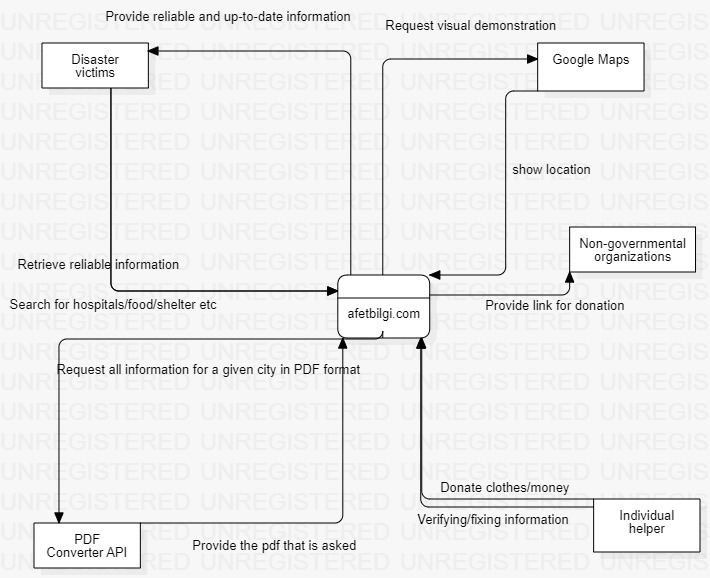
\includegraphics[scale=0.5]{context-diagram}
    \centering
    \caption{Context diagram}
\end{figure}

\subsubsection*{System Interfaces}
Using Google Maps API to show where important information is located. Integration with
social media sites for sharing information. APIs are used for getting data from external 
sources like pharmacies and hospitals.

\subsubsection*{User Interfaces}
User-friendly interface for language and location-based information search with filtering system
for the best viewing experience across many platforms, including desktops, laptops, tablets, and
smartphones, using responsive design. Users have the choice to download reliable information PDFs
for cities for offline use.

\subsubsection*{Software Interfaces}
Using Google Maps API integration to display locations. Information is shared through integration
with social media platforms. PDF Converter API is used to enable users download reliable and up-to-date
information about cities for offline use. Language translation API is used to make website more accessible to 
speakers of other languages.

\subsubsection*{Communication Interfaces}
Provide links for donation and help for individuals/non-governmental organizations. HTTPS protocol 
is used to exchange data with the end-user, including payment and personal information.

\subsubsection*{Memory Constraints}
Since visitors could only have a limited amount of internet connectivity in an emergency, the
website is optimized for quick loading and low bandwidth usage. To ensure that it can be accessible
on low-end devices, the website is built to use the least amount of RAM possible.

\subsubsection*{Operations}
User operations: Search for hospitals, shelter locations, gathering places and pharmacies etc.
View details on pharmacies, hospitals, gathering places, and shelters. Filter the website with one of
the provided languages. Download PDFs

Admin operations: Update the website frequently with the most recent details and information. Create regular
website backups for a server failure.

Overall operations: Maintaining the website often to keep it up-to-date and functional. The website
is optimized for quick loading and low bandwidth usage. Information that is sent by users should
be verified and added to system.

\subsection{External Interfaces}

\begin{figure}[H]
    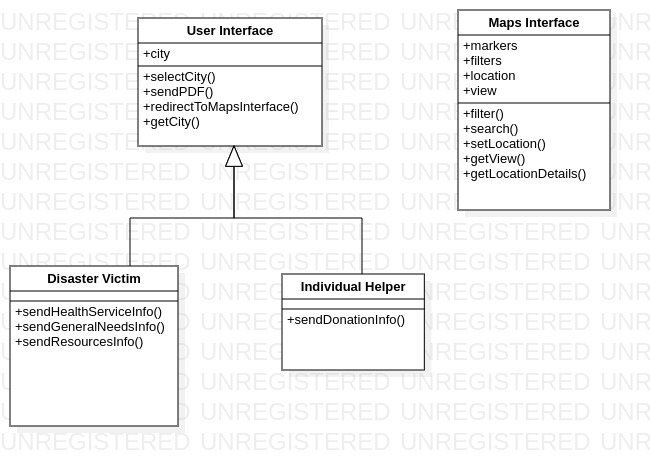
\includegraphics[scale=0.5]{ext1}
    \centering
    \caption{External Interfaces}
\end{figure}

The user interface is the primary external interface of afetbilgi.com and serves as the interaction point between the website and its users. The functions of the user interface include:
\begin{itemize}
    \item Information Retrieval: Users can access critical information about the disaster, including details about hospitals, assembly points, shelter locations, and pharmacies. They can retrieve and view this information through the user interface.

    \item Filtering by City: The user interface allows users to filter the available information based on their city. This functionality enables users to focus on the resources and locations relevant to their specific location and needs.

    \item Donations and Contributions: The user interface provides users with the ability to donate and offer support to the affected areas or relief efforts. It allows users to contribute their resources, time, or updated information to help improve the accuracy and availability of the provided data.

    \item Search Functionality: The user interface includes a search feature that enables users to easily search for specific information they need. Users can search for specific hospitals, assembly points, shelter locations, or other resources, making it convenient to find the desired information quickly.
\end{itemize}

The Google Maps interface is an external interface integrated into afetbilgi.com, enhancing the functionality and user experience. The functions of the Google Maps interface include:

\begin{itemize}
    \item Visualization of Information: The Google Maps interface allows users to visually explore the available information on a map. It provides a spatial representation of hospitals, assembly points, shelter locations, and other resources, making it easier for users to understand their locations in relation to their surroundings.

    \item Interactive Map Navigation: Users can interact with the Google Maps interface to zoom in/out, pan, and explore different areas. They can navigate through the map to find specific locations, get directions, or determine proximity to resources.

    \item Location-based Search: The Google Maps interface enables users to perform location-based searches. Users can input their current location or desired destination, and the interface will display relevant resources and locations in that area.

    \item Integration with Information: The Google Maps interface is integrated with the underlying information of afetbilgi.com. Users can click on map markers or specific areas to access detailed information about the corresponding resources, such as hospital details or shelter availability.
\end{itemize}

\subsection{Interaction Scenarios}
\begin{figure}[H]
    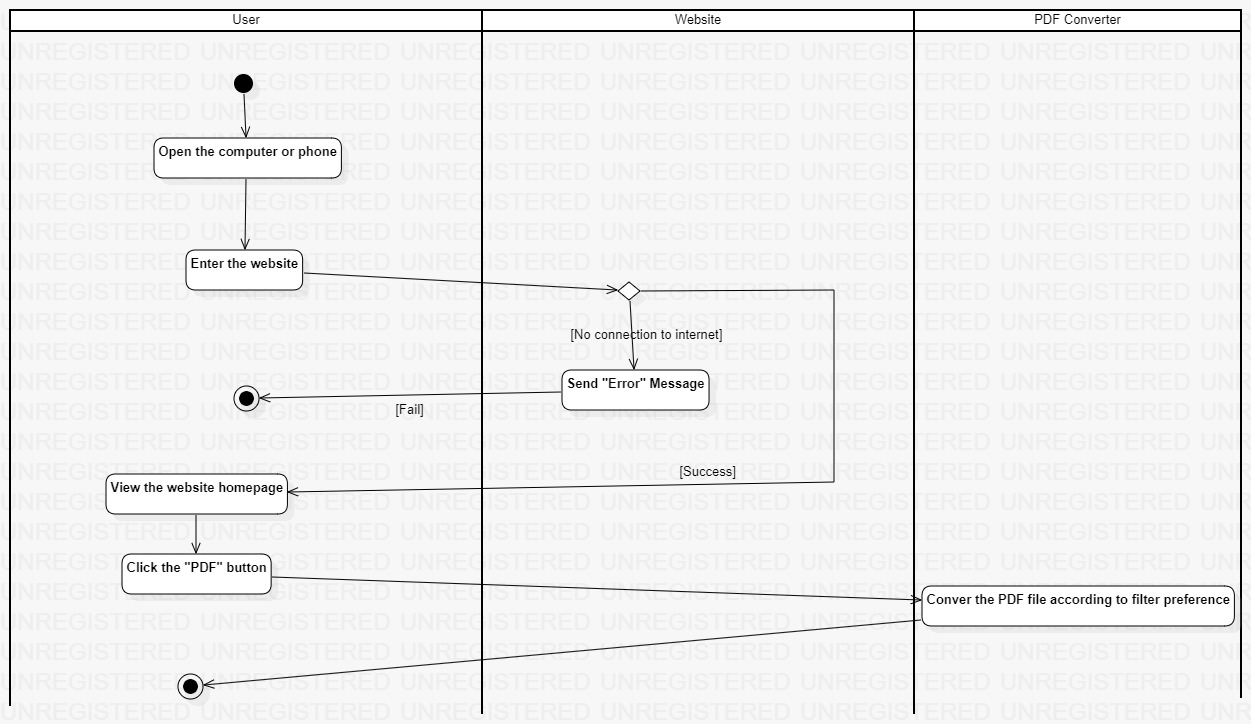
\includegraphics[scale=0.4]{act1.jpg}
    \centering
    \caption{Activity diagram for PDF generation}
\end{figure}

\begin{figure}[H]
    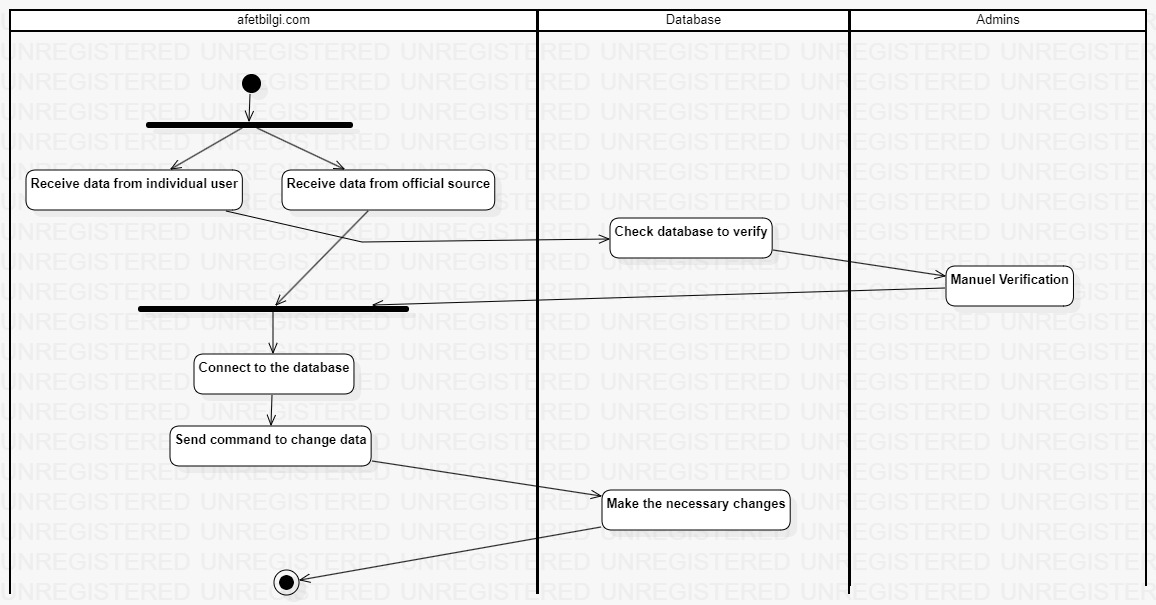
\includegraphics[scale=0.4]{act2.jpg}
    \centering
    \caption{Activity diagram for updating data}
\end{figure}

\section{Functional View}

\subsection{Stakeholders' uses of this view}
The functional view of afetbilgi.com caters to the needs of multiple stakeholders. Users can easily navigate the website, access critical information, 
and utilize filtering options for efficient searches. Website administrators gain a comprehensive understanding of the website's features, enabling 
effective management and decision-making. Individual helpers and donors understand how to update data and contribute to the cause, while service providers
can ensure accurate representation of their facilities. Overall, the functional view enhances user experience, facilitates website management, encourages 
active participation, and promotes seamless information retrieval and support during disasters.

\subsection{Component Diagram}
\begin{figure}[H]
    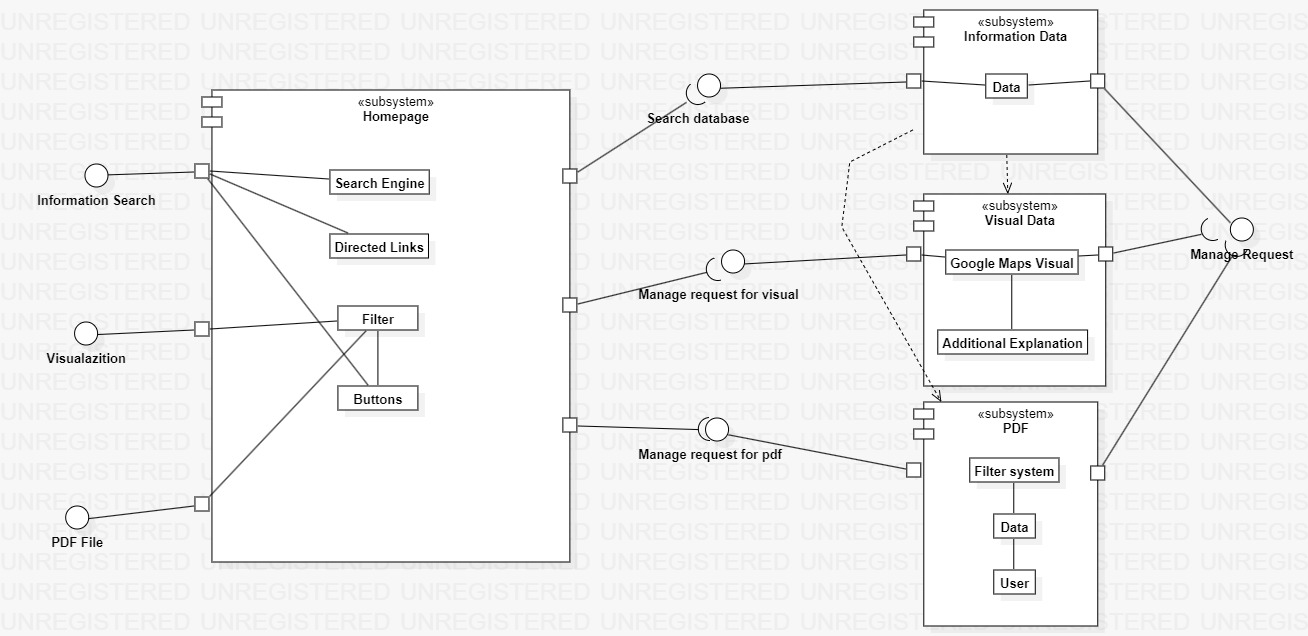
\includegraphics[scale=0.4]{component1.jpg}
    \centering
    \caption{Component Diagram}
\end{figure}

There are four subsystems in afetbilgi.com, Homepage, Data server which consists of 3 parts: Information Data, Visual Data, PDF Data.
Homepage consists of Search Engine, Directed Links, Filter, and Buttons.
The website provides searching information on the website according to the filters, with the search engine, directed links and buttons.
The website provides visualizing the locations of shelters, gathering places, utilities etc for the user with an interface, called Visualization with Google Maps API.
The website provides the PDF file for the cities containing important information for the related cities by using PDF Converter API.
Information Data contains all the written information in the Data base to use it in converting PDF or adding extra information to google maps visuals.
Visual Data gathers the visuals from Google Maps and adds the necessary information according to the design of the developers. 
The PDF system takes the information from data base with filtering according to the chosen city and converts it to a PDF form.
Information search calls “search database” which will show the related information if it exists.
Visualization calls “search database” to verify it exists and “manage request for visual” to show the visual of the data asked to the user.
PDF File calls “search database” to verify it exists and “manage request for pdf” to provide the pdf form of the data asked.
After reviewing the request from the user, the system manages the request accordingly.

\subsection{Internal Interfaces}
\begin{figure}[H]
    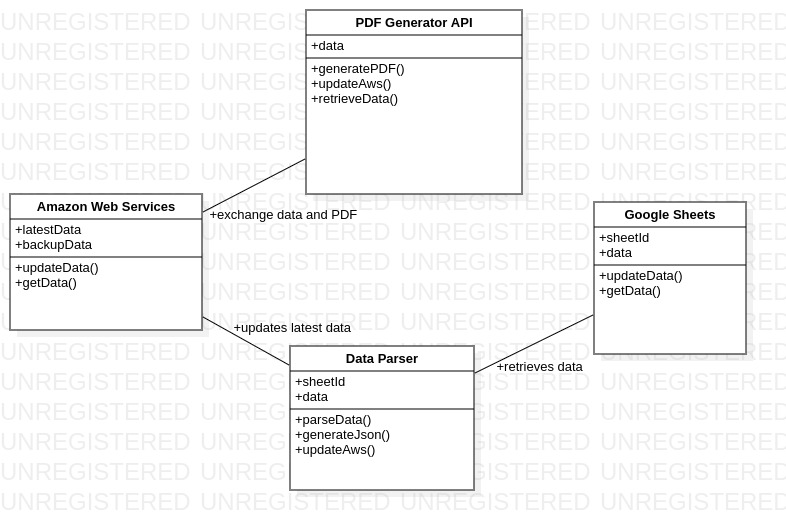
\includegraphics[scale=0.5]{internal1.jpg}
    \centering
    \caption{Internal Interfaces}
\end{figure}

\subsection{Interaction Patterns}

\begin{figure}[H]
    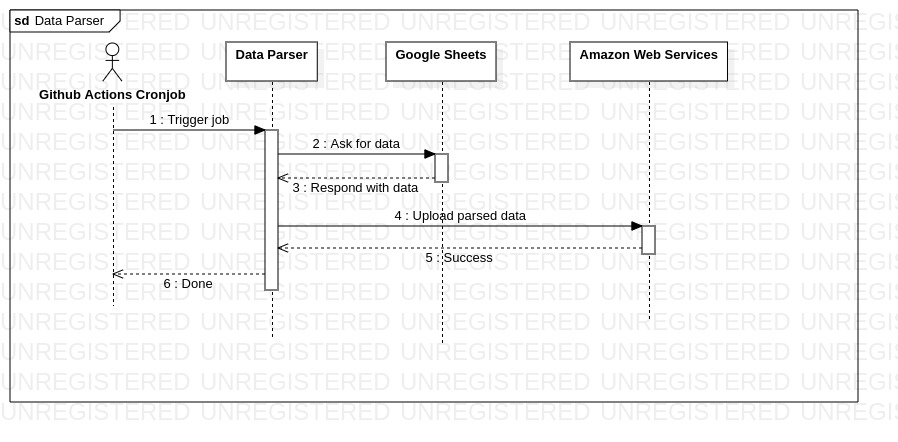
\includegraphics[scale=0.6]{seq1.jpg}
    \centering
    \caption{Sequence diagram for data parsing}
\end{figure}


\begin{figure}[H]
    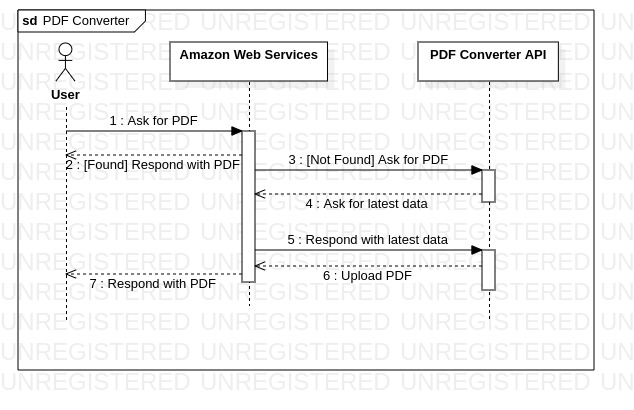
\includegraphics[scale=0.6]{seq2.jpg}
    \centering
    \caption{Sequence diagram for PDF converter}
\end{figure}

\begin{figure}[H]
    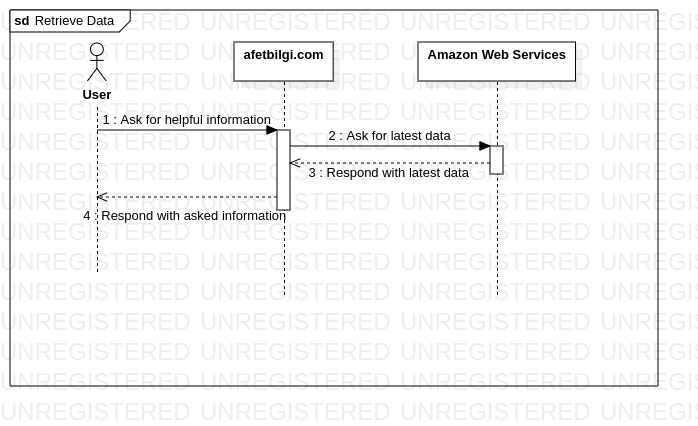
\includegraphics[scale=0.6]{seq3.jpg}
    \centering
    \caption{Sequence diagram for retrieving information}
\end{figure}

\section{Information View}

\subsection{Stakeholders' uses of this view}
The information view in afetbilgi.com serves multiple stakeholders. Users benefit by easily accessing relevant information such as 
hospitals, assembly points, shelters, and donation centers. Website administrators utilize the information view to organize and manage 
different types of data. Service providers ensure their data is accurately represented. Overall, the information view enhances user navigation, aids 
website management, facilitates coordination among stakeholders, and ensures accurate and accessible information during disaster situations.

\subsection{Database Class Diagram}
\begin{figure}[H]
    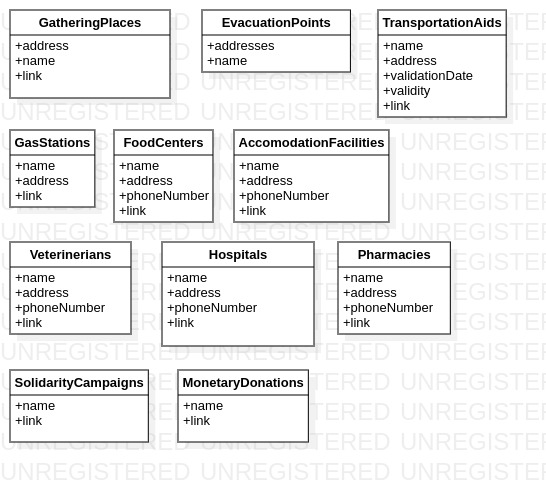
\includegraphics[scale=0.6]{db1}
    \centering
    \caption{Database class diagram}
\end{figure}

\subsection{Operations on Data}
\renewcommand{\arraystretch}{2}
\begin{table}[H]
    \centering
    \begin{tabular}{|l|p{10cm}|}
        \hline
    \textbf{Operation}             & \textbf{Description} \\ \hline
    Gathering Place            & Create / update / remove / read gathering place \\ \hline
    Accomodation Facility      & Create / update / remove / read accomodation facility  \\ \hline
    Evacuation Point           & Create / update / remove / read evacuation point \\ \hline
    Food Center                & Create / update / remove / read food center \\ \hline
    Gas Station                & Create / update / remove / read gas station \\ \hline
    Transportation Aid         & Create / update / remove / read transportation aid \\ \hline
    Hospital                   & Create / update / remove / read hospital \\ \hline
    Veterinerian               & Create / update / remove / read veterinerian \\ \hline
    Pharmacy                   & Create / update / remove / read pharmacy \\ \hline
    Solidarity Campaigns       & Create / update / remove / read solidarity campaigns \\ \hline
    Monetary Donation          & Create / update / remove / read monetary donation \\ \hline
    \end{tabular}
    \caption{Database operations}
\end{table}

\section{Deployment View}

\subsection{Stakeholders' uses of this view}
The deployment view in afetbilgi.com facilitates effective planning, monitoring, and collaboration for website administrators, 
developers, system administrators, and the infrastructure team, ensuring a robust and reliable deployment.

\subsection{Deployment Diagram}
\begin{figure}[H]
    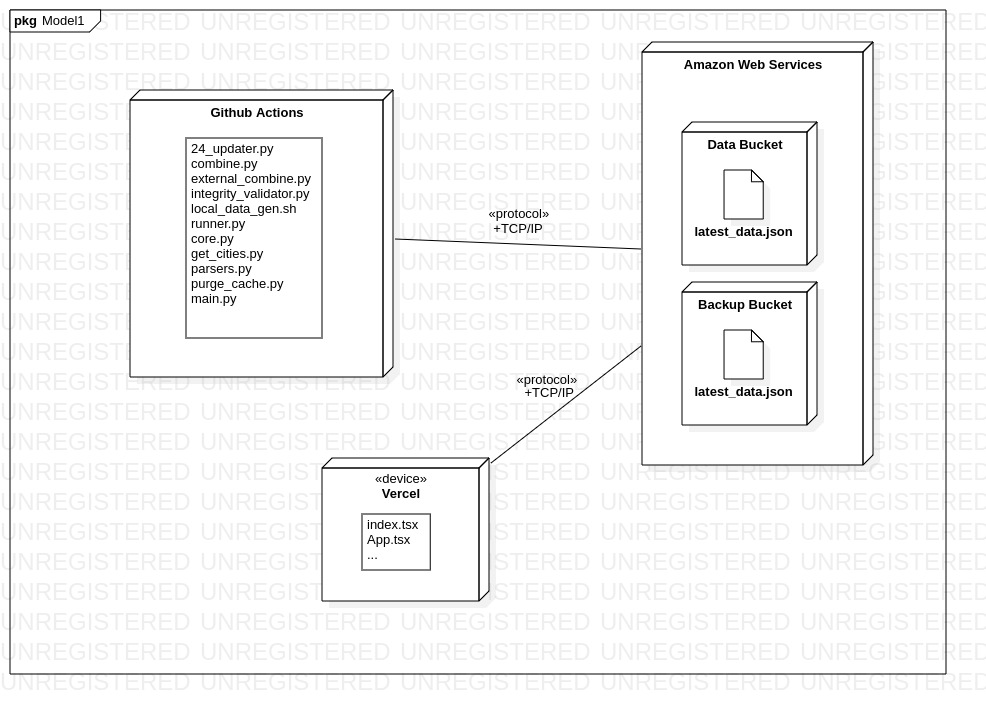
\includegraphics[scale=0.5]{deploy1}
    \centering
    \caption{Deployment Diagram}
\end{figure}

afetbilgi.com is deployed using a combination of technologies to ensure efficient data processing, storage, and hosting. The deployment includes the following components:
\begin{itemize}
    \item Github Actions: Continuous integration and deployment platform that automates the execution of data parsing scripts on a scheduled basis.

    \item AWS Data Buckets: Cloud storage solution used to store the parsed data in JSON format, providing reliable and scalable storage for the information.

    \item Vercel Servers: Hosting platform for the front end of afetbilgi.com, ensuring fast and reliable content delivery to users.
\end{itemize}
    

This deployment setup enables regular updates of information, secure data storage, and a responsive user experience.

\section{Design Rationale}
The design rationale for the context view in afetbilgi.com revolves around providing stakeholders with a clear understanding of the website's purpose, facilitating alignment, improving user experience, guiding system development and maintenance, supporting data integration and verification, and enabling scalability and adaptability.
\newline

The design rationale for the functional view in afetbilgi.com is to create a user-friendly system that provides easy access to critical information, promotes collaboration, and encourages disaster preparedness.
\newline

The design rationale for the information view in afetbilgi.com is to organize and present information effectively for easy access and accurate representation.
\newline

The design rationale for the deployment view in afetbilgi.com is to ensure a robust and efficient system deployment.

\chapter{Architectural Views for Suggestion to Improve the Existing System}

\section{Context View}

\subsection{Stakeholders' uses of this view}
The suggested improvements in integrating with municipalities' building database, implementing advanced filtering for PDF generation, 
and enabling user-generated information sharing enhance the stakeholders' uses of the context view in afetbilgi.com. Users gain access to accurate 
building status information, customizable PDF generation, and real-time insights from other users. Administrators can oversee the integration process 
and facilitate user contributions. Municipalities and non-governmental organizations benefit from reliable information and enhanced coordination. Overall, 
these enhancements strengthen the system's effectiveness and usefulness.

\subsection{Context Diagram}

\begin{figure}[H]
    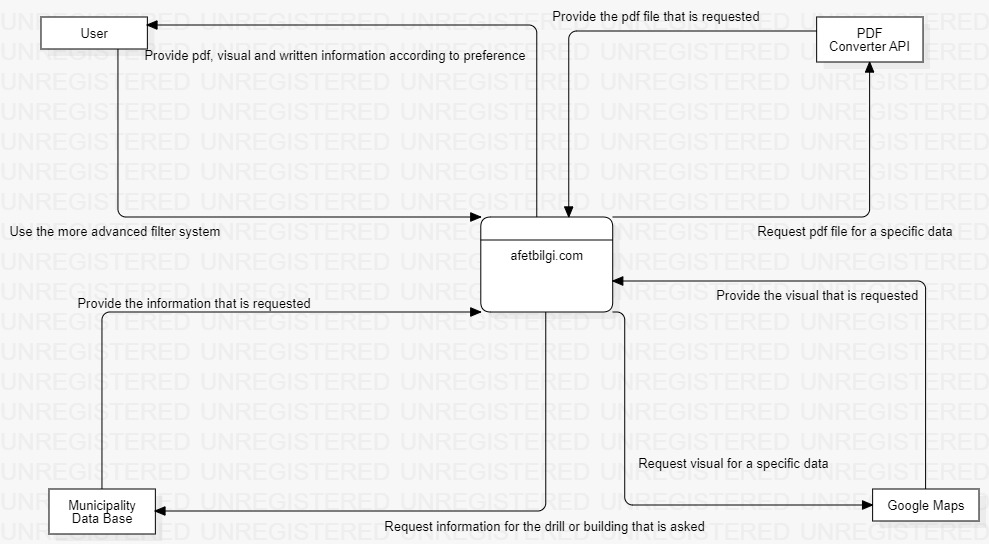
\includegraphics[scale=0.5]{context2}
    \centering
    \caption{Context diagram suggestion}
\end{figure}

\subsubsection{System Interfaces}
Using Google Maps, PDF Converter API and Municipality Data Base to provide related and up-to-date information. APIs are also used for getting data from external sources.

\subsubsection{User Interfaces}
Easier to use and find the related information with advanced filter system so that they can reach or get the pdf file also for specific information. Regulating the screen size according to the device that is connected to the server. Users can use pdf files offline too. Users can also upload data to the system and wait for its verification.

\subsubsection{Software Interfaces}
Using Google Maps API integration to visualize the locations according to the search of the user. PDF Converter API is used to give the pdf file that user asked information with filter. REST API to provide information through the website of Municipality.

\subsubsection{Communication Interfaces}
Provide links for donations and help for individuals/non-governmental organizations. HTTPS protocol is used to exchange data with the end-user, including payment and personal information.

\subsubsection{Memory Constraints}
Memory Constraints Since visitors could only have a limited amount of internet connectivity in an emergency, the website is optimized for quick loading and low bandwidth usage. To ensure that it can be accessible on low-end devices, the website is built to use the least amount of RAM possible.

\subsubsection{Operations}
User operations: Use the advanced filter to search for specific information and get the pdf file for it. Upload data and wait for its verification.

Admin operations: Update the website frequently with the most recent details and information. Create regular website backups for a server failure. Check for the data that is uploaded by users and verify it.

Overall operations: Maintaining the website often to keep it up-to-date and functional. The website is optimized for quick loading and low bandwidth usage. Information that is sent by users should be verified and added to the system.

\subsection{External Interfaces}
\begin{figure}[H]
    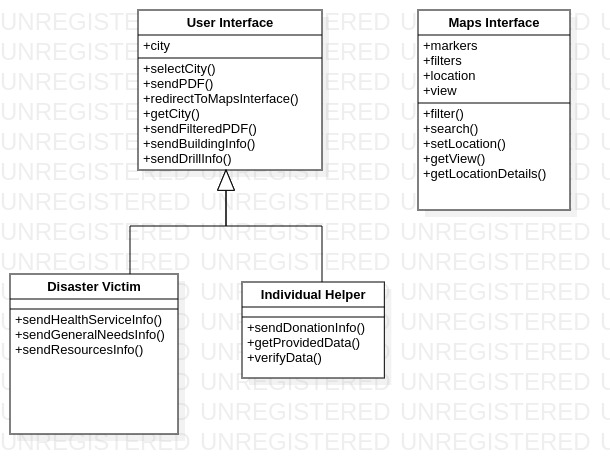
\includegraphics[scale=0.6]{ext2.jpg}
    \centering
    \caption{External interfaces suggestions}
\end{figure}

User Interface:
\begin{itemize}
    \item User-friendly platform for stakeholders to retrieve critical disaster information.
    \item Easy access and filtering of information by city for quick and relevant data retrieval.
    \item Integration with municipalities' building database to provide building status and strength information.
    \item User contribution feature for sharing updates and information, enhancing the available data.
    \item Individual helpers can donate and offer assistance through the interface, promoting community involvement and support.
\end{itemize}

Google Maps Interface:
\begin{itemize}
    \item Integration of Google Maps for enhanced visualization and usability.
    \item Interactive maps to view and inspect disaster-related information.
    \item Filtering and search capabilities for efficient location of points of interest.
    \item Integration with municipalities' building database to assess building strength and status on the map.
\end{itemize}

\subsection{Interaction Scenarios}
\begin{figure}[H]
    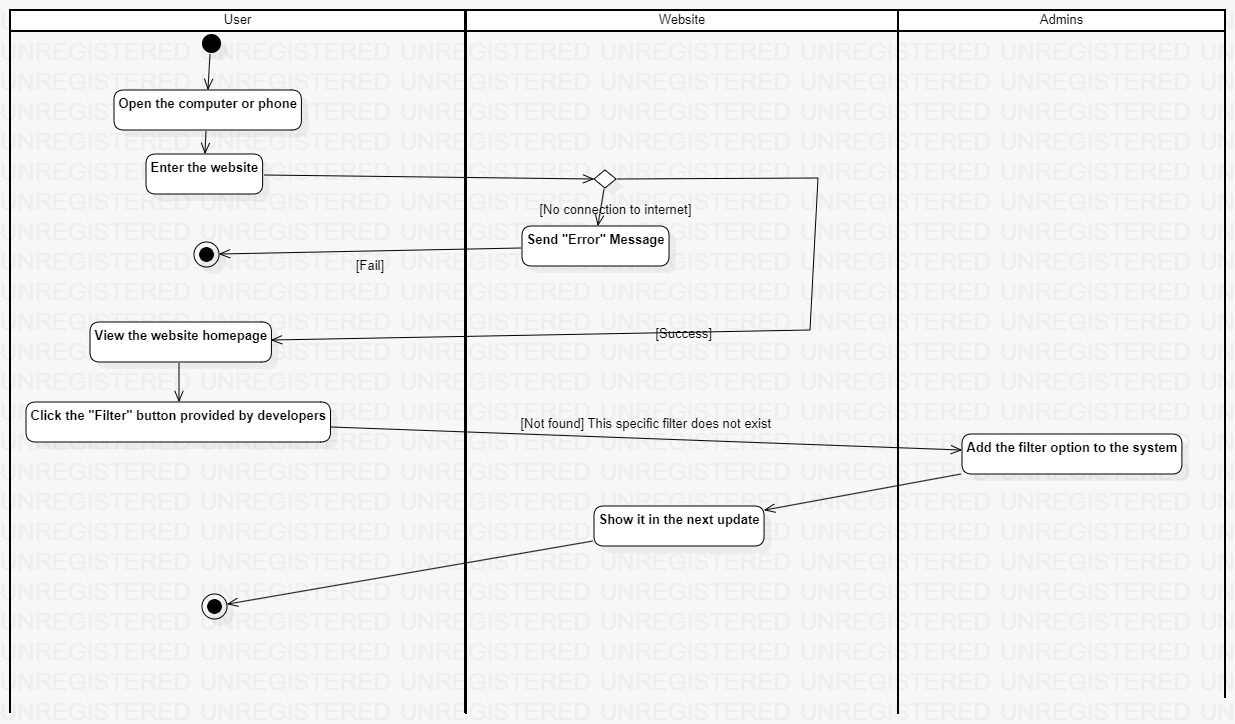
\includegraphics[scale=0.4]{actsuggestion.jpg}
    \centering
    \caption{Activity diagram suggestion}
\end{figure}

\section{Functional View}

\subsection{Stakeholders' uses of this view}
The stakeholders' uses of the functional view, considering the suggested improvements, include accessing accurate and personalized information for 
users, overseeing and managing the system's expanded functionalities for administrators, verifying and contributing building status information for
municipalities and government authorities. The functional view serves a vital interface that empowers stakeholders to leverage the system's capabilities, 
collaborate, and contribute towards improved disaster management.

\subsection{Component Diagram}
\begin{figure}[H]
    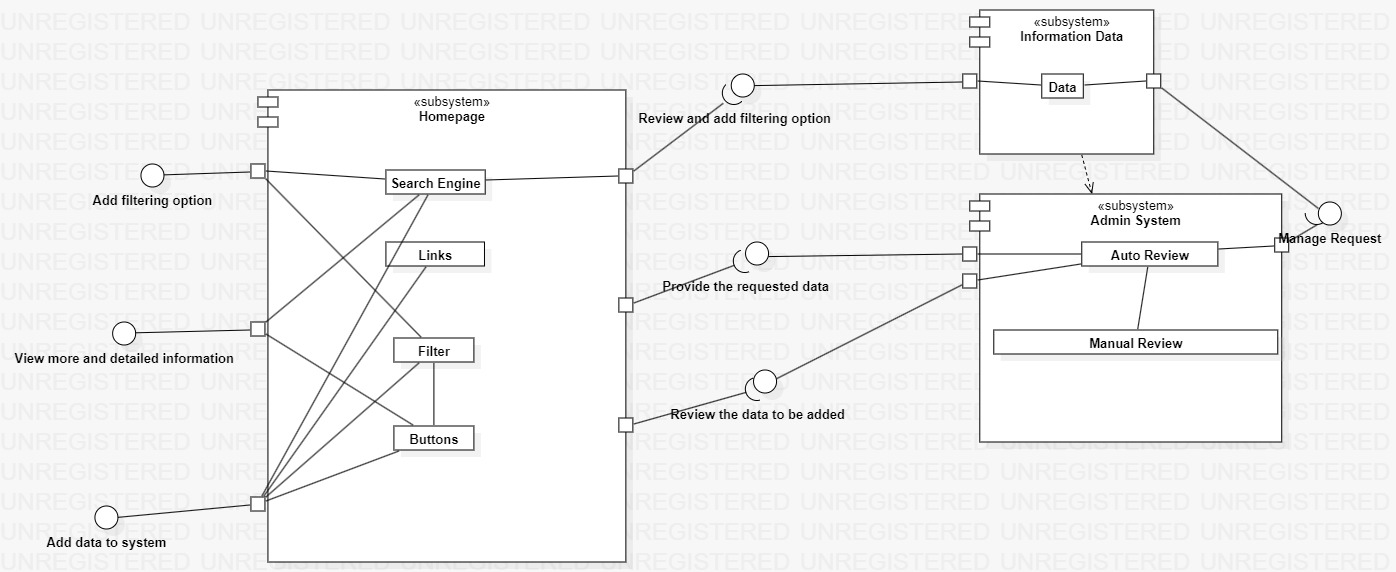
\includegraphics[scale=0.4]{component2.jpg}
    \centering
    \caption{Component diagram suggestion}
\end{figure}

There are three subsystems needed for the suggestions in afetbilgi.com, Homepage, Data server (Information Data) and Admin System	
Homepage consists of Search Engine, Directed Links, Filter, and Buttons.
The website provides an interface to the user to add a new filtering option to the website.
The website provides more and detailed information to the user with preference of the user(Drill information/ building earthquake tests etc.)
The website provides an interface called Add data to system, which enables individual users to add data which is not on the website yet.
Information Data contains all the written information in the Data base to verify the data or use it in converting PDF or adding extra information to google maps visuals.
Admin System has auto review and manual review.
Auto review is developed by admins to see if it is something considered before and is decided as not to appear. 
Manual review is for admins to manually review it if nothing comes from auto review.
Add filtering option calls “review and add filtering options” which will check the data base to see if it exists, if not, send it to admin system.
View more and detailed information is for users to share their opinions with the admins about the website so that admins can show detailed information about other topics related to emergencies in the website.
Adding data to system calls “review the data to be added” which will send it to admins to verify this information and decide if this information would be useful.
After reviewing the request from the user, the system manages the request accordingly.


\subsection{Internal Interfaces}
\begin{figure}[H]
    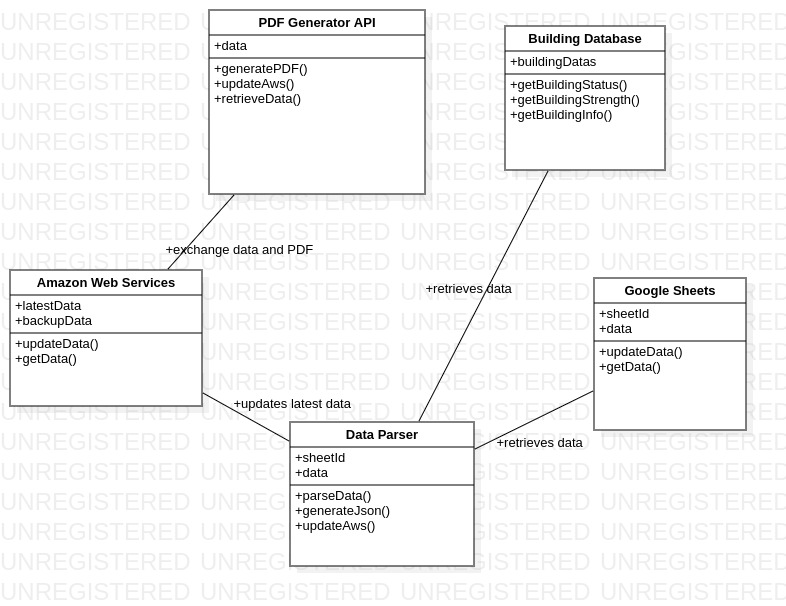
\includegraphics[scale=0.6]{internal2.jpg}
    \centering
    \caption{Internal interfaces suggestion}
\end{figure}

\subsection{Interaction Patterns}
\begin{figure}[H]
    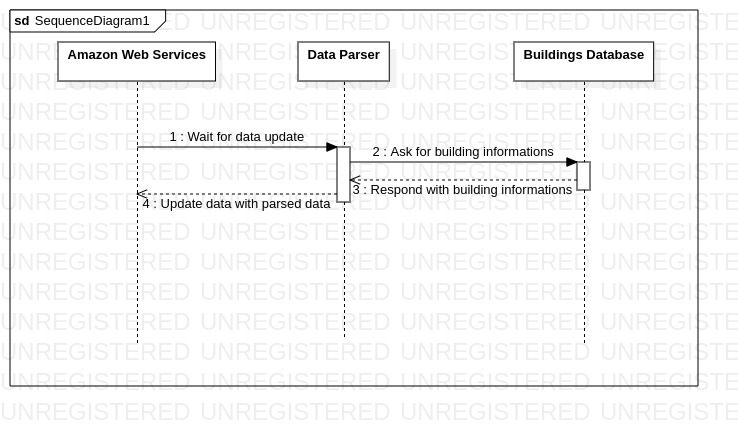
\includegraphics[scale=0.6]{seqsuggest}
    \centering
    \caption{Suggestion for sequence diagram for data parsing}
\end{figure}

\section{Information View}

\subsection{Stakeholders' uses of this view}
The stakeholders' uses of the information view, considering the suggested improvements, include accessing comprehensive and accurate information 
for users, organizing and presenting integrated data for administrators, verifying and disseminating reliable information for municipalities and 
government authorities. The information view serves as a crucial component that empowers stakeholders with relevant, timely, and reliable information, 
enhancing their decision-making and response capabilities during disasters.

\subsection{Database Class Diagram}
\begin{figure}[H]
    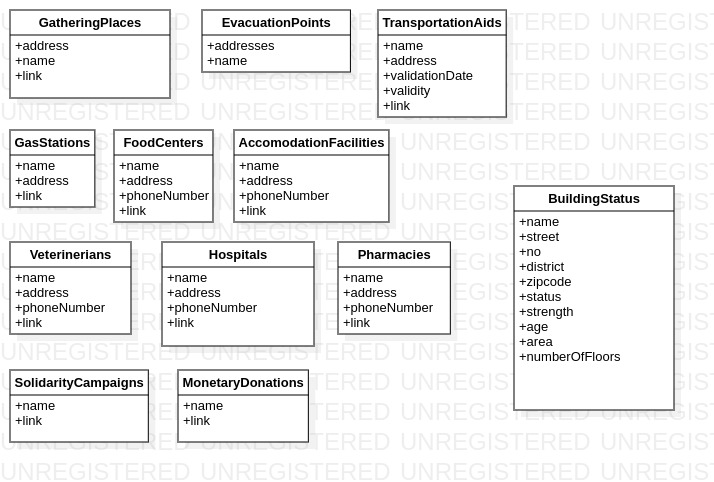
\includegraphics[scale=0.6]{db2}
    \centering
    \caption{Database class diagram suggestion}
\end{figure}

\subsection{Operations on Data}
\begin{table}[H]
    \centering
    \begin{tabular}{|l|p{10cm}|}
        \hline
    \textbf{Operation}             & \textbf{Description} \\ \hline
    Gathering Place            & Create / update / remove / read gathering place \\ \hline
    Accomodation Facility      & Create / update / remove / read accomodation facility  \\ \hline
    Evacuation Point           & Create / update / remove / read evacuation point \\ \hline
    Food Center                & Create / update / remove / read food center \\ \hline
    Gas Station                & Create / update / remove / read gas station \\ \hline
    Transportation Aid         & Create / update / remove / read transportation aid \\ \hline
    Hospital                   & Create / update / remove / read hospital \\ \hline
    Veterinerian               & Create / update / remove / read veterinerian \\ \hline
    Pharmacy                   & Create / update / remove / read pharmacy \\ \hline
    Solidarity Campaigns       & Create / update / remove / read solidarity campaigns \\ \hline
    Monetary Donation          & Create / update / remove / read monetary donation \\ \hline
    Buildings                  & Read building informations \\ \hline
    \end{tabular}
    \caption{Database operations suggestion}
\end{table}
\section{Deployment View}

\subsection{Stakeholders' uses of this view}
The stakeholders' uses of the deployment view, considering the suggested improvements, include accessing reliable and customizable information for users,
managing the smooth integration of databases for administrators and municipalities. The deployment view ensures that the system's features 
and functionalities are effectively implemented and made available to stakeholders, contributing to the overall effectiveness and usability of afetbilgi.com during disaster situations.

\subsection{Deployment Diagram}
\begin{figure}[H]
    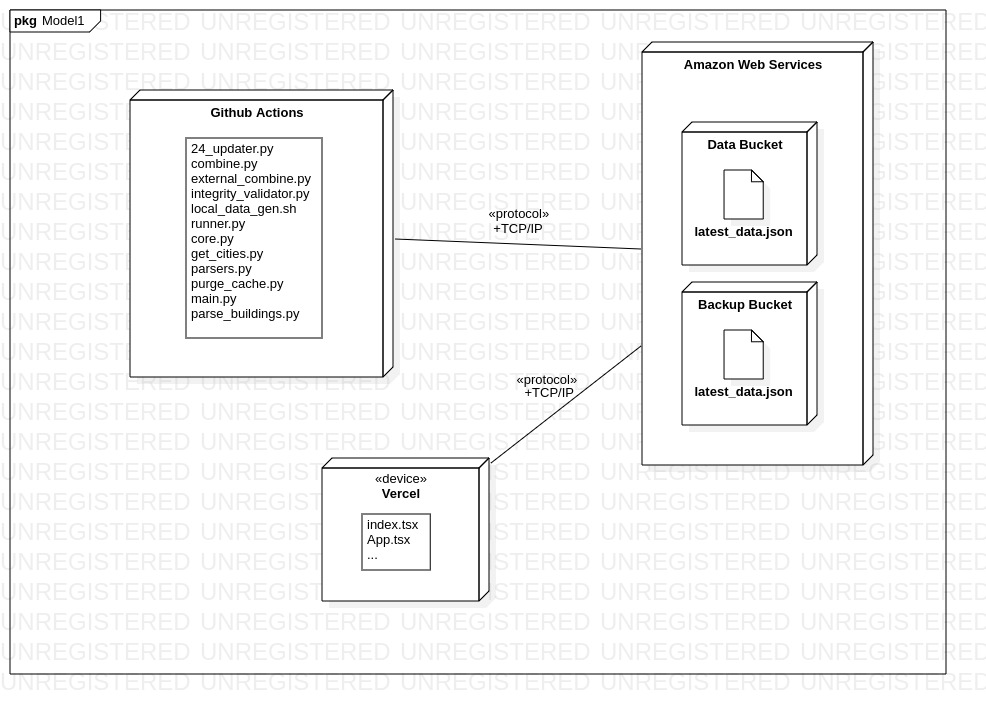
\includegraphics[scale=0.5]{deploy2}
    \centering
    \caption{Deployment Diagram Suggestion}
\end{figure}

Apart from the original deployment scheme, only change is the new Python script (parse\_buildings.py) which is responsible for parsing building data retrieved from the integrated municipality database.

\section{Design Rationale}
The Context View aims to provide stakeholders with a comprehensive understanding of the system's environment. Integration with municipalities' building database ensures accurate building status information. Advanced filtering allows users to customize retrieved information, and user-generated sharing enhances collaboration.
\newline

The Functional View aligns system functionalities with stakeholder needs. Integration with building database enables seamless retrieval of accurate data. Advanced filtering offers flexibility, and user-generated sharing promotes real-time information exchange.
\newline

The Information View presents a clear and organized representation of system information. Integration with building database ensures comprehensive and reliable data. Advanced filtering enhances usability, and user-generated sharing enriches available information.
\newline

The Deployment View focuses on efficient implementation and utilization of system features. Integration with building database enables seamless access to building status information.

\end{document}